%-------------------------------------------------------------------------------
%-------------------------------------------------------------------------------
\begin{frame}\begin{center}
\LARGE\textbf{Internal rate of return}
\end{center}\end{frame}
%-------------------------------------------------------------------------------
%-------------------------------------------------------------------------------
\begin{frame}
We study two different concepts of the rate of return in schooling:

\vspace{0.3cm}
\begin{itemize}\setlength\itemsep{1em}
\item marginal differences
\item non-marginal differences\vspace{0.3cm}
\end{itemize}

We treat schooling as a continuous choice initially but then account for its discrete nature.

\end{frame}
%-------------------------------------------------------------------------------
%-------------------------------------------------------------------------------
\begin{frame}
\textbf{Income Maximization under Perfect Certainty \nocite{Rosen.1977,Willis.1979}}
\begin{align*}
s               &\qquad\text{schooling level} \\
x               &\qquad\text{experience level} \\
Y(s, x)         &\qquad\text{wage income} \\
T(s)            &\qquad\text{last age of earnings} \\
v               &\qquad\text{tuition and psychic cost of schooling} \\
\tau            &\qquad\text{proportional tax rate} \\
r               &\qquad\text{before-tax interest rate}
\end{align*}
\end{frame}
%-------------------------------------------------------------------------------
%-------------------------------------------------------------------------------
\begin{frame}
\textbf{Present Discounted Value of Lifetime Earnings}
\begin{align*}
V(s) = & \int_0^{T(s) - s} (1 - \tau) e^{-(1 - \tau)r(x + s)} Y(s,x) dx \\
       & - \int^s_0 ve^{-(1 - \tau)rz}dz
\end{align*}
\end{frame}
%-------------------------------------------------------------------------------
%-------------------------------------------------------------------------------
\begin{frame}
First-Order Condition
\begin{align*}
& [T^\prime(s) - 1]e^{-(1 - \tau)r(T(s) - s)} Y(s, T(s) - s) \\
& - (1 - \tau)r\int^{T(s) - s}_0 e^{-(1 - \tau)rx} Y(s, x)dx \\
& + \int_0^{T(s) - s} e^{-(1 - \tau) rx} \frac{\partial Y(s, x)}{\partial s}dx \\
& - \frac{v}{ 1  -\tau} = 0
\end{align*}
\end{frame}
%-------------------------------------------------------------------------------
%-------------------------------------------------------------------------------
\begin{frame}
Rearranging and defining $\tilde{r} = (1 - \tau)r$ ...
\begin{align}
\tilde{r} & = \frac{[T^\prime(s) - 1]e^{-\tilde{r}(T(s) - s)}Y(s, T(s) - s )}{\int_0^{T(s) - s} e^{-\tilde{r}x}Y(s, x) dx} \\
          & + \frac{\int_0^{T(s) - s}e^{-\tilde{r}x}\left[\frac{\partial Y(s, x)}{\partial s}\right] dx}{\int_0^{T(s) - s}e^{-\tilde{r}x}Y(s, x) dx} \\
          & - \frac{\frac{v}{1-\tau}}{\int_0^{T(s) - s}e^{-\tilde{r}x}Y(s, x)dx}
\end{align}
\end{frame}
%-------------------------------------------------------------------------------
%-------------------------------------------------------------------------------
\begin{frame}\textbf{Interpretation}\vspace{0.3cm}
\begin{itemize}\setlength\itemsep{1em}
\item (1) ... the change in the present value of earnings due to a change in working-life with additional schooling
\item (2) ... weighted average effect of schooling on log earnings by experience
\item (3) ... tuition and psychic costs\vspace{0.3cm}
\end{itemize}

All components are expressed as a fraction of the present value of earnings measured at age $s$
\end{frame}
%-------------------------------------------------------------------------------
%-------------------------------------------------------------------------------
\begin{frame}\textbf{Getting back to Mincer}\vspace{0.3cm}
\begin{itemize}\setlength\itemsep{1em}
\item no tuition and psychic costs of schooling \\
    $\qquad\Rightarrow v = 0$
\item no loss of working life from schooling \\
    $\qquad\Rightarrow T^\prime(s) = 1$
\item multiplicative separability between schooling and experience component of earnings \\
    $\qquad\Rightarrow Y(s, x) = \mu(s)\psi(x)$
\end{itemize}
\end{frame}
%-------------------------------------------------------------------------------
%-------------------------------------------------------------------------------
\begin{frame}
\begin{align*}
\tilde{r} = \frac{\mu^\prime(s)}{\mu(s)}\quad\forall\quad s\\
\end{align*}

Thus, wage growth must be log linear in schooling and $\mu(s) = \mu(0)e^{\rho_s s}$ and $\tilde{r} = \rho_s$.

\end{frame}
%-------------------------------------------------------------------------------
%-------------------------------------------------------------------------------
\begin{frame}\textbf{Structural Approach for the IRR}\vspace{0.3cm}\\

The internal rate of return for schooling level $s_1$ versus $s_2$, $r_I(s_1, s_2)$ solves ...

\begin{align*}
&\int_{0}^{T(s_1) - s_1} (1 - \tau)e^{-r_I(x + s_1)}Y(s_1, x) dx  - \int_{0}^{s_1} v e^{-r z} dz\\
&\qquad\qquad =  \int_{0}^{T(s_2) - s_2} (1 - \tau)e^{-r_I(x + s_2)}Y(s_2, x) dx - \int_{0}^{s_2} v e^{-r z} dz
\end{align*}

\end{frame}
%-------------------------------------------------------------------------------
%-------------------------------------------------------------------------------
\begin{frame}
Back to Mincer ....

\begin{itemize}
\item no taxes and no direct or psychic costs of schooling \\\vspace{0.3cm}
\hspace{0.3cm}$\Rightarrow v = 0$ and $\tau = 0$\vspace{0.3cm}
\begin{align*}
&\int_{0}^{T(s_1) - s_1} e^{-r_I(x + s_1)}Y(s_1, x) dx  = \int_{0}^{T(s_2) - s_2} e^{-r_I(x + s_2)}Y(s_2, x) dx
\end{align*}
\end{itemize}\end{frame}
%-------------------------------------------------------------------------------
%-------------------------------------------------------------------------------
\begin{frame}
\begin{itemize}
\item equal work-lives irrespective of years of schooling \\\vspace{0.3cm}
\hspace{0.3cm}$\Rightarrow T = T(s_1) - s_1 = T(s_2) - s_2$\vspace{0.3cm}
\begin{align*}
&\int_{0}^T e^{-r_I(x + s_1)}Y(s_1, x) dx  = \int_{0}^T e^{-r_I(x + s_2)}Y(s_2, x) dx
\end{align*}
\end{itemize}
\end{frame}
%-------------------------------------------------------------------------------
%-------------------------------------------------------------------------------
\begin{frame}
\begin{itemize}
\item parallelism in experience across schooling categories \\\vspace{0.3cm}
\hspace{0.3cm}$\Rightarrow Y(s, x) = \mu(s)\psi(x)$\vspace{0.3cm}
\begin{align*}
&\int_{0}^T e^{-r_I(x + s_1)} \mu(s)\psi(x) dx  = \int_{0}^T e^{-r_I(x + s_2)} \mu(s)\psi(x)dx
\end{align*}
\end{itemize}
\end{frame}
%-------------------------------------------------------------------------------
%-------------------------------------------------------------------------------
\begin{frame}
\begin{itemize}
\item linearity of log earnings in schooling \\\vspace{0.3cm}
\hspace{0.3cm}$\Rightarrow\quad \mu(s) = \mu(0)e^{\rho_s s}$\vspace{0.3cm}
\begin{align*}
&\int_{0}^T e^{-r_I(x + s_1)} \mu(0)e^{\rho_s s_1}\psi(x) dx  = \int_{0}^T e^{-r_I(x + s_2)} \mu(0)e^{\rho_s s_2}\psi(x)dx
\end{align*}
\end{itemize}
\end{frame}
%-------------------------------------------------------------------------------
%-------------------------------------------------------------------------------
\begin{frame}
After some further rearranging ...
\begin{align*}
e^{(\rho_s - r_I)s_1} & = e^{(\rho_s - r_I) s_2} \\
\Rightarrow \rho_s  & = r_I
\end{align*}
\end{frame}
%-------------------------------------------------------------------------------
%-------------------------------------------------------------------------------
\begin{frame}
\citeA{Heckman.2006a} thus establish ... \vspace{0.5cm}

\begin{quote}
After allowing for taxes, tuition, variable length of working life, and a flexible relationship between earnings, schooling and experience, the coefficient on years of schooling in a log earnings regression need no longer equal the internal rate of return.
\end{quote}
\end{frame}
%-------------------------------------------------------------------------------
%-------------------------------------------------------------------------------
\begin{frame}\begin{center}
\LARGE\textit{Empirical Evidence}
\end{center}\end{frame}
%-------------------------------------------------------------------------------
%-------------------------------------------------------------------------------
\begin{frame}\textbf{Specifications}\vspace{0.3cm}
\begin{itemize}\setlength\itemsep{1em}
\item \textbf{relax linearity in $S$}, including indicator variables for each level of schooling
\item \textbf{relax linearity and parallelism}, nonparametrically estimated functions of experience, separately within each schooling level
\end{itemize}
\end{frame}
%-------------------------------------------------------------------------------
%-------------------------------------------------------------------------------
\begin{frame}[plain]
\begin{center}
\scalebox{0.5}{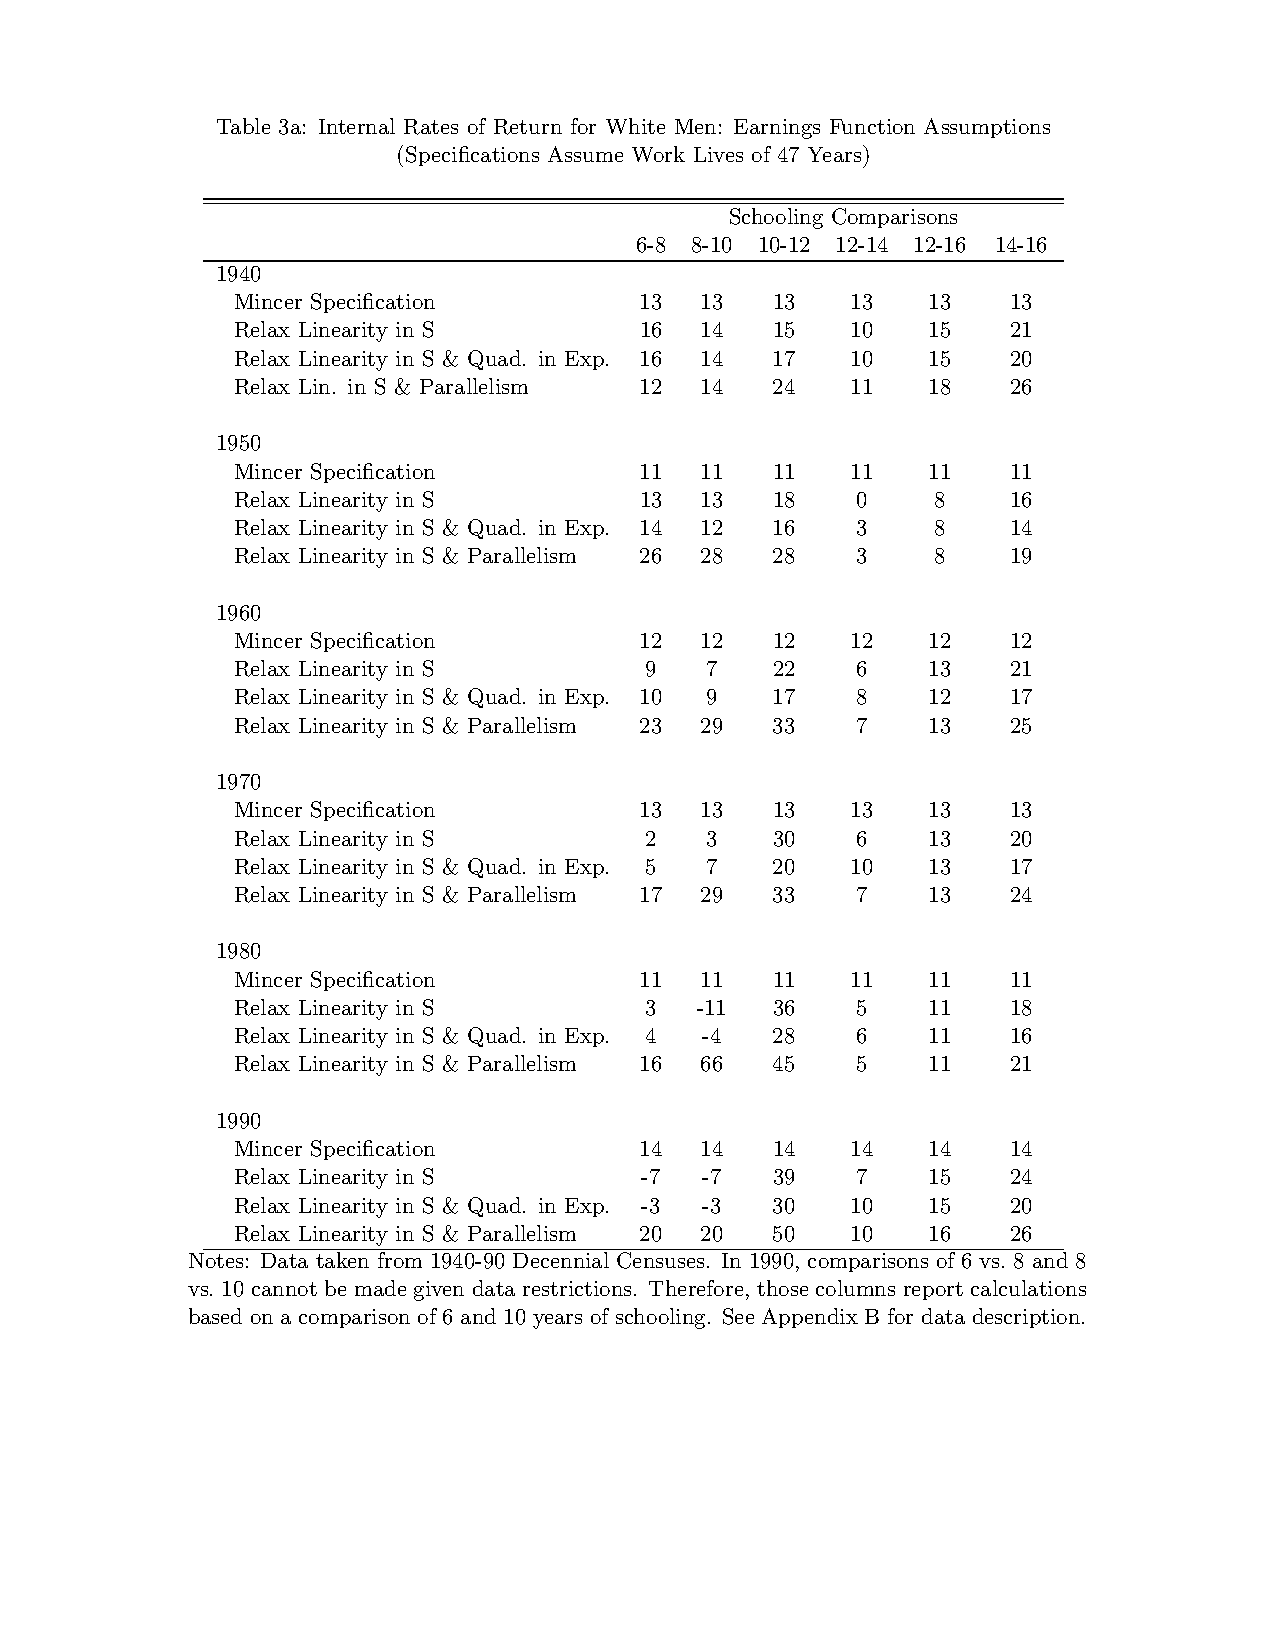
\includegraphics{tab-irr-specifications-white}}
\end{center}
\end{frame}
%-------------------------------------------------------------------------------
%-------------------------------------------------------------------------------
\begin{frame}[plain]
\begin{center}
\scalebox{0.5}{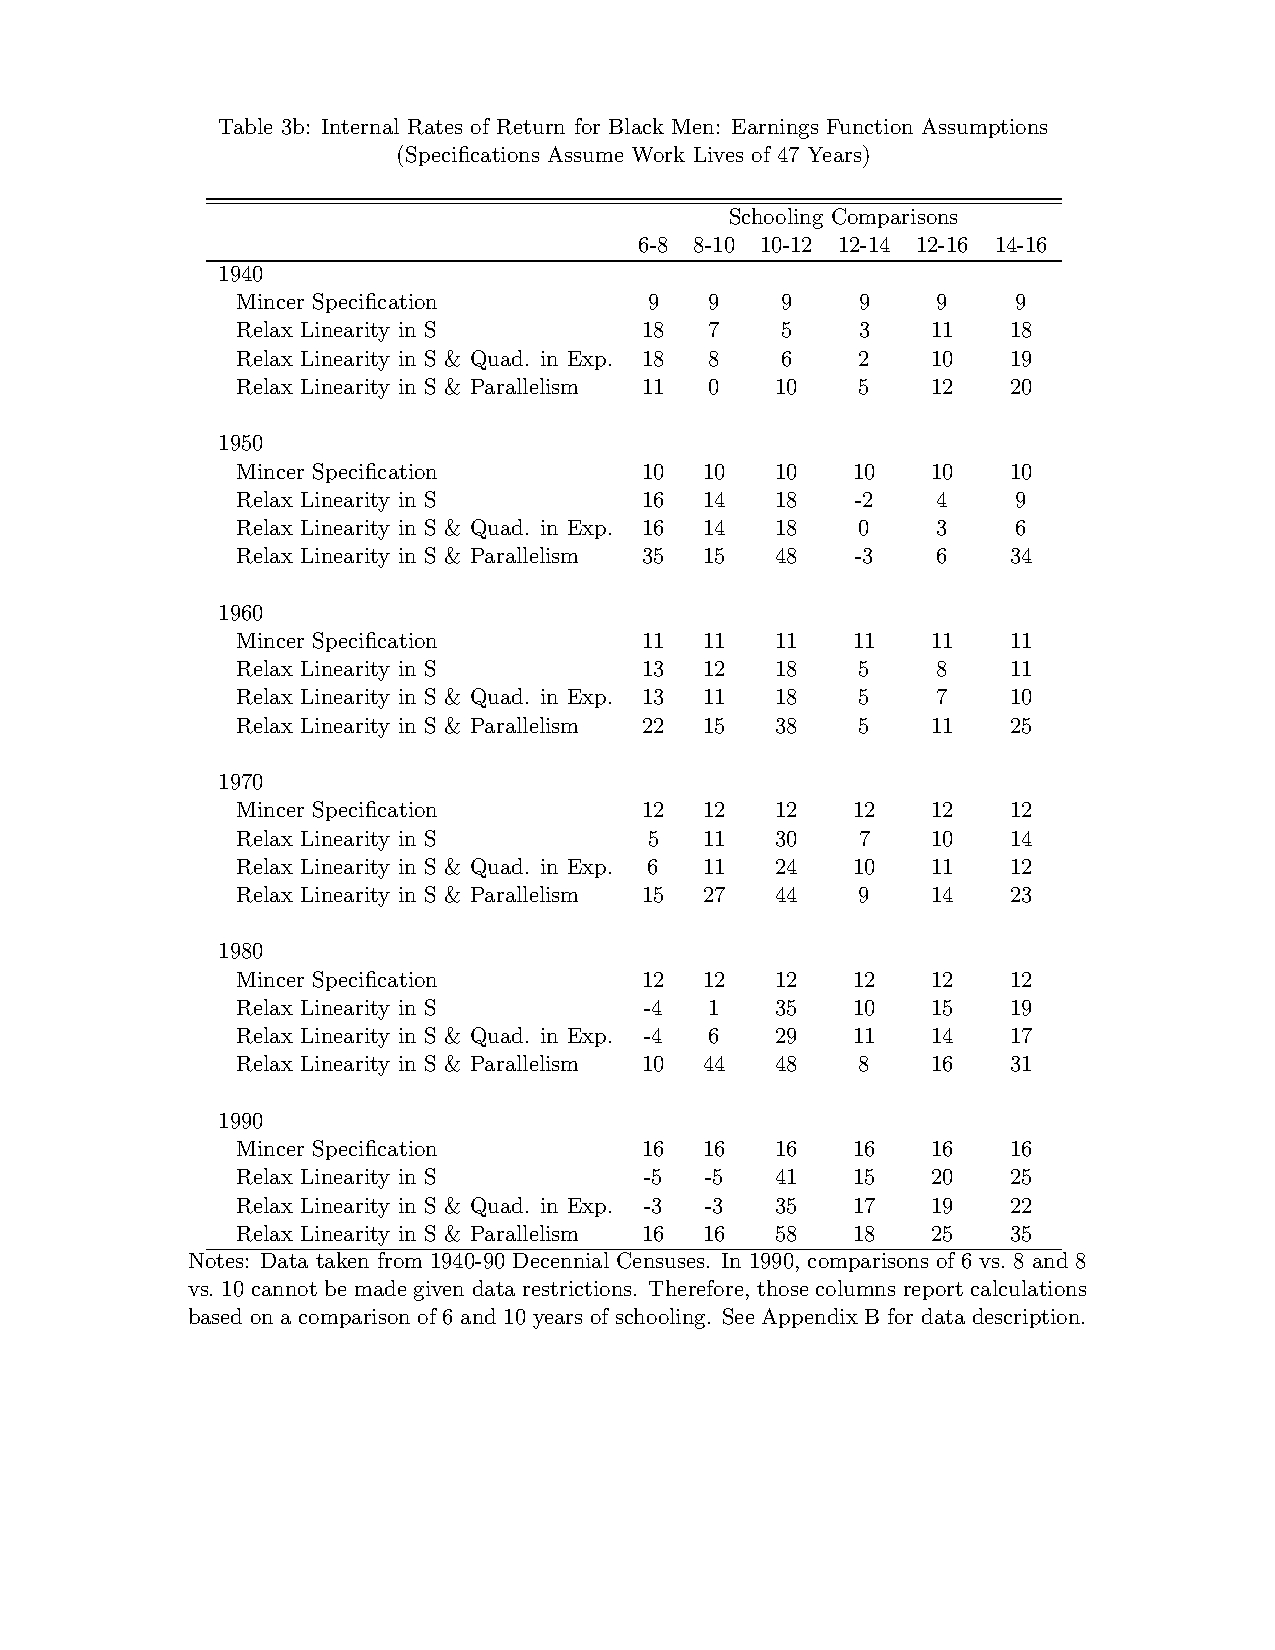
\includegraphics{tab-irr-specifications-black}}
\end{center}
\end{frame}
%-------------------------------------------------------------------------------
%-------------------------------------------------------------------------------
\begin{frame}[plain]
\begin{center}
\scalebox{0.5}{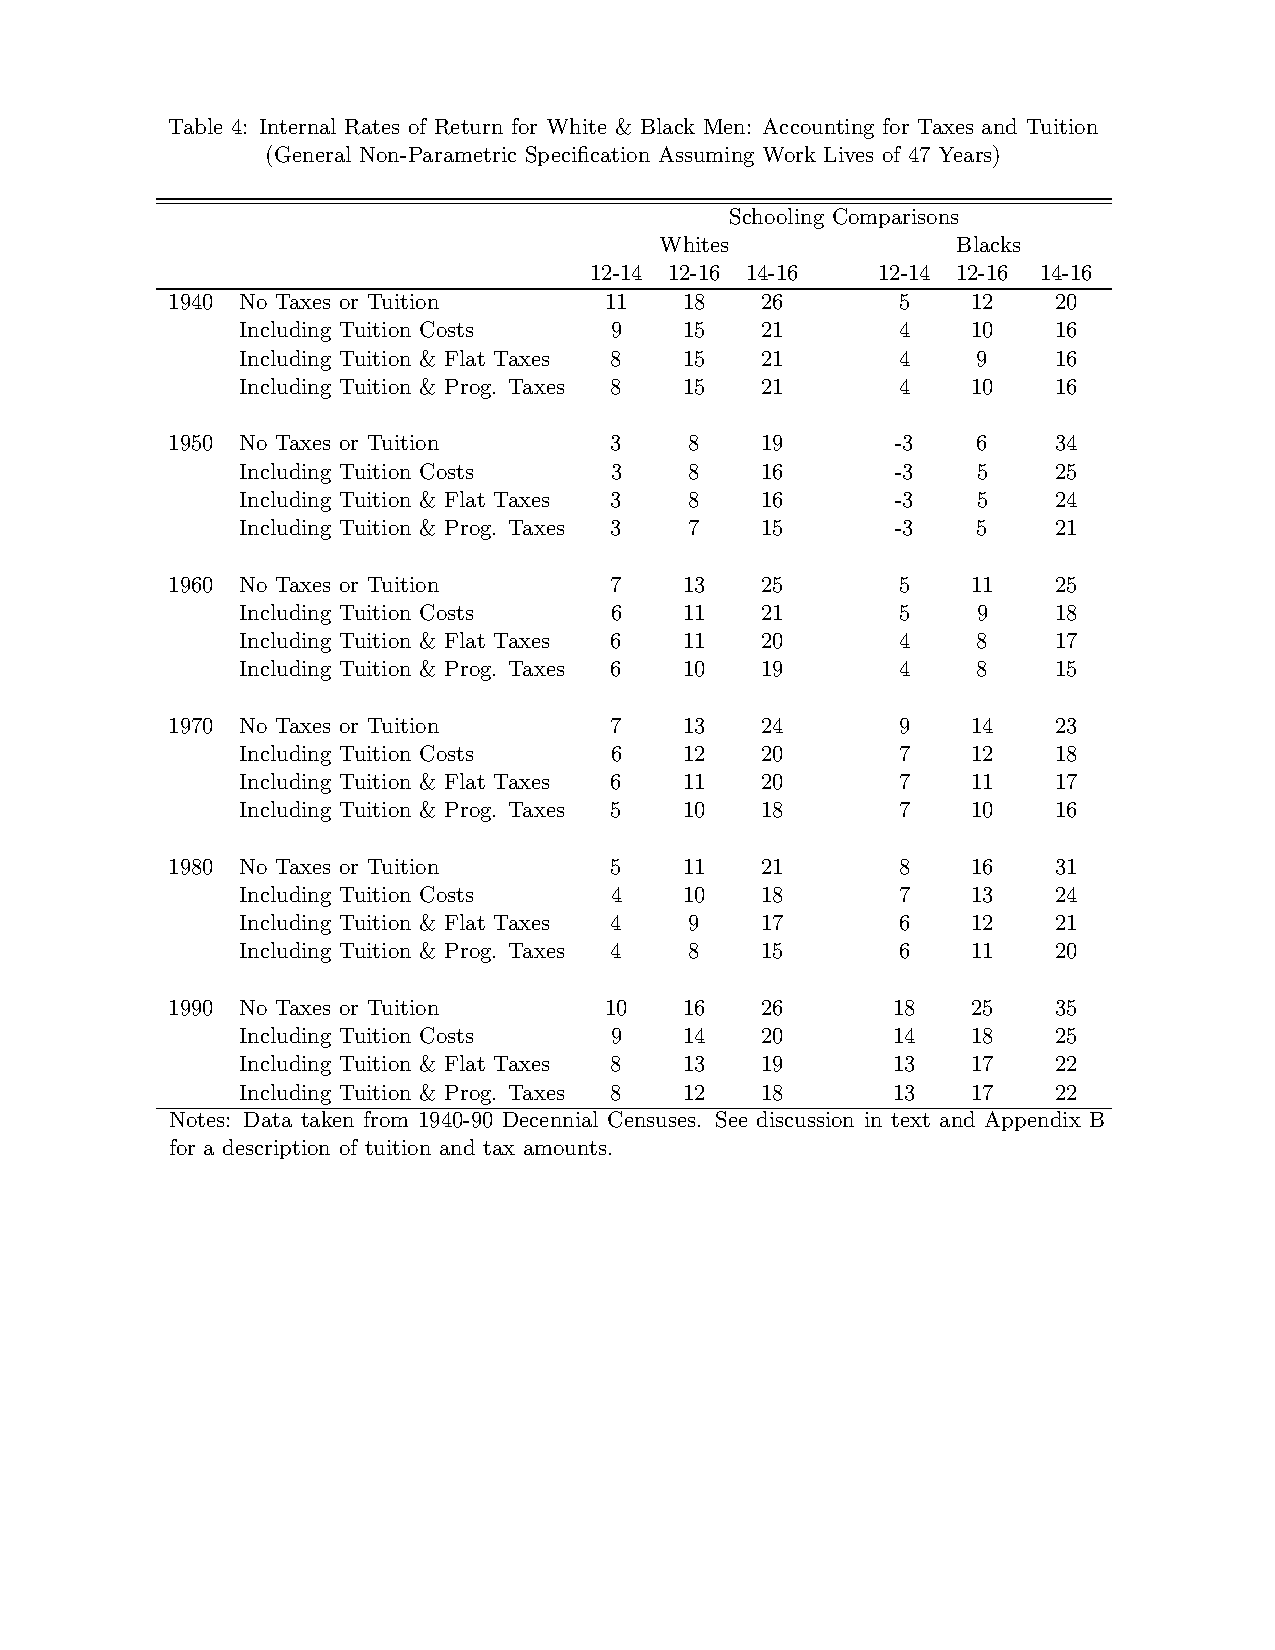
\includegraphics{tab-irr-specifications-cost}}
\end{center}
\end{frame}
%-------------------------------------------------------------------------------
%-------------------------------------------------------------------------------
\begin{frame}[plain]
\begin{center}
\scalebox{0.75}{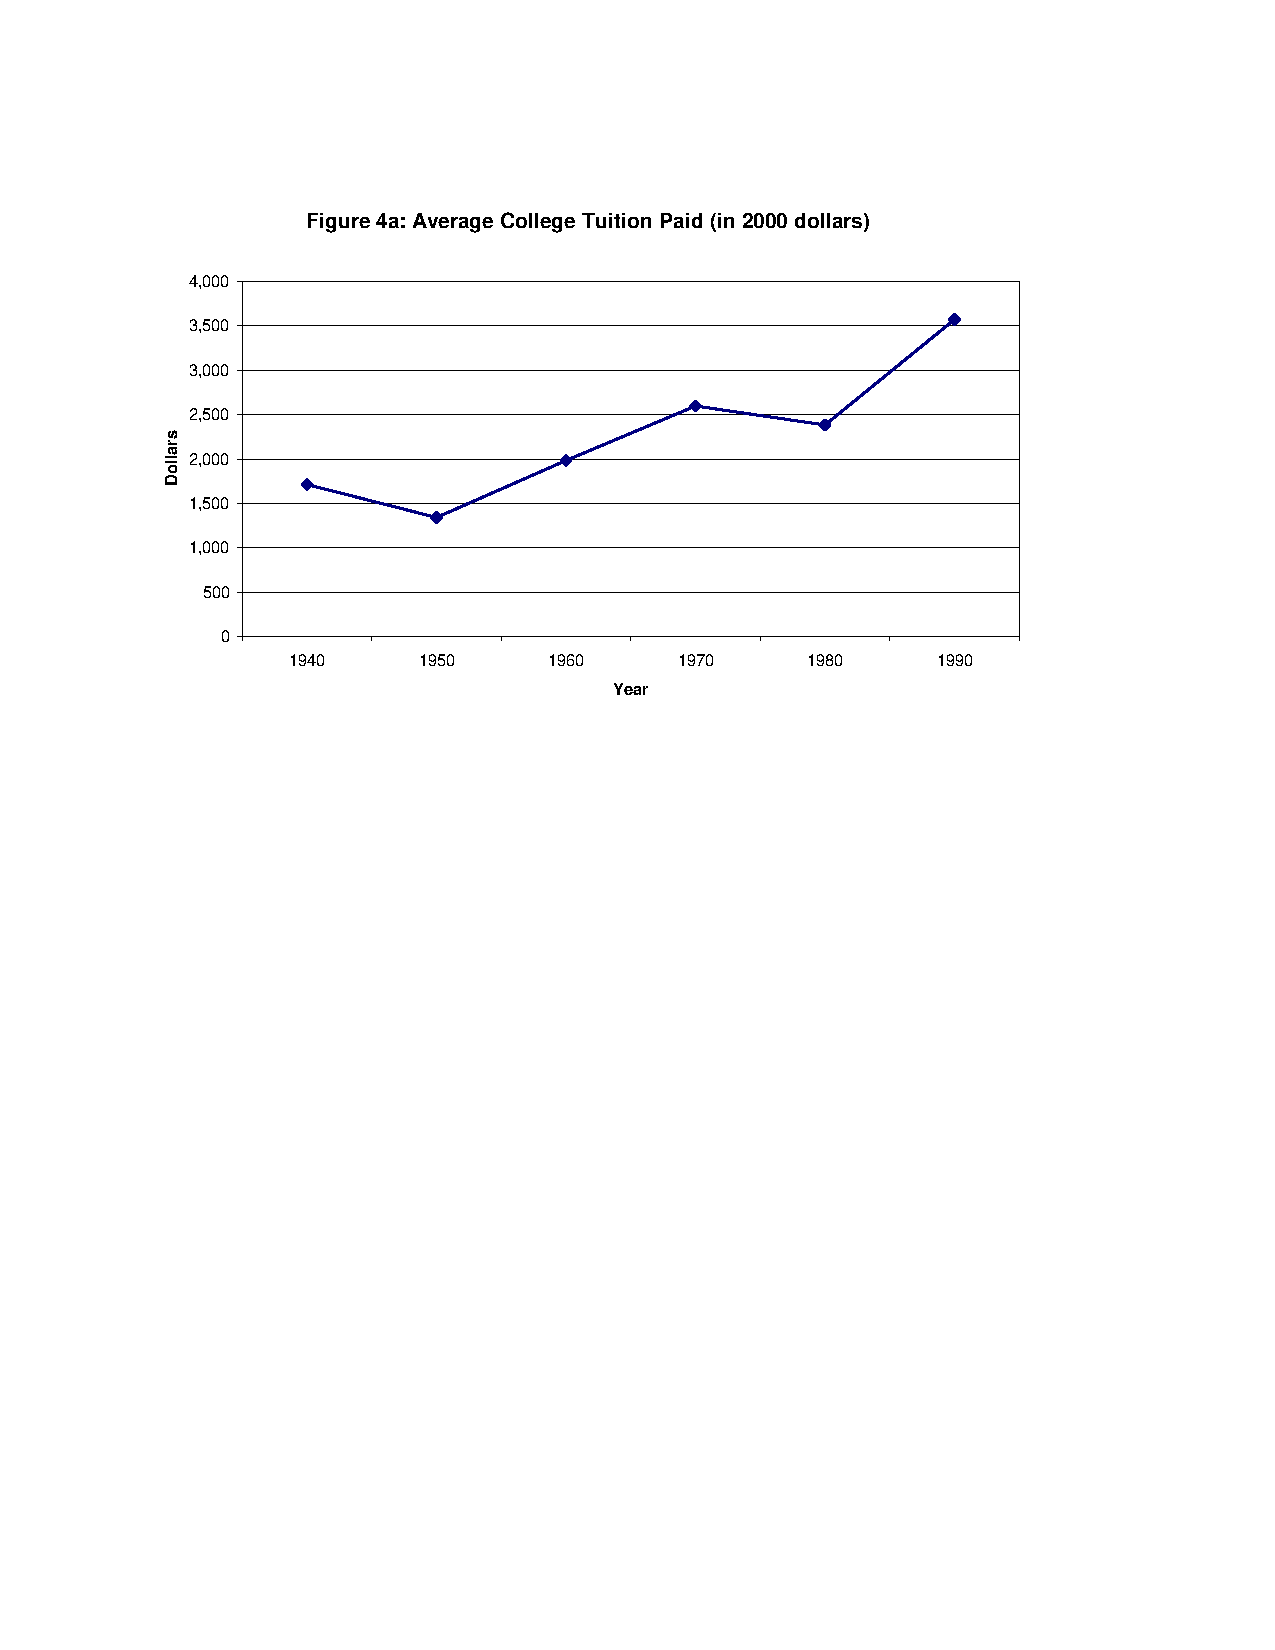
\includegraphics{fig-college-tuition}}
\end{center}
\end{frame}
%-------------------------------------------------------------------------------
%-------------------------------------------------------------------------------
\begin{frame}[plain]
\begin{center}
\scalebox{0.75}{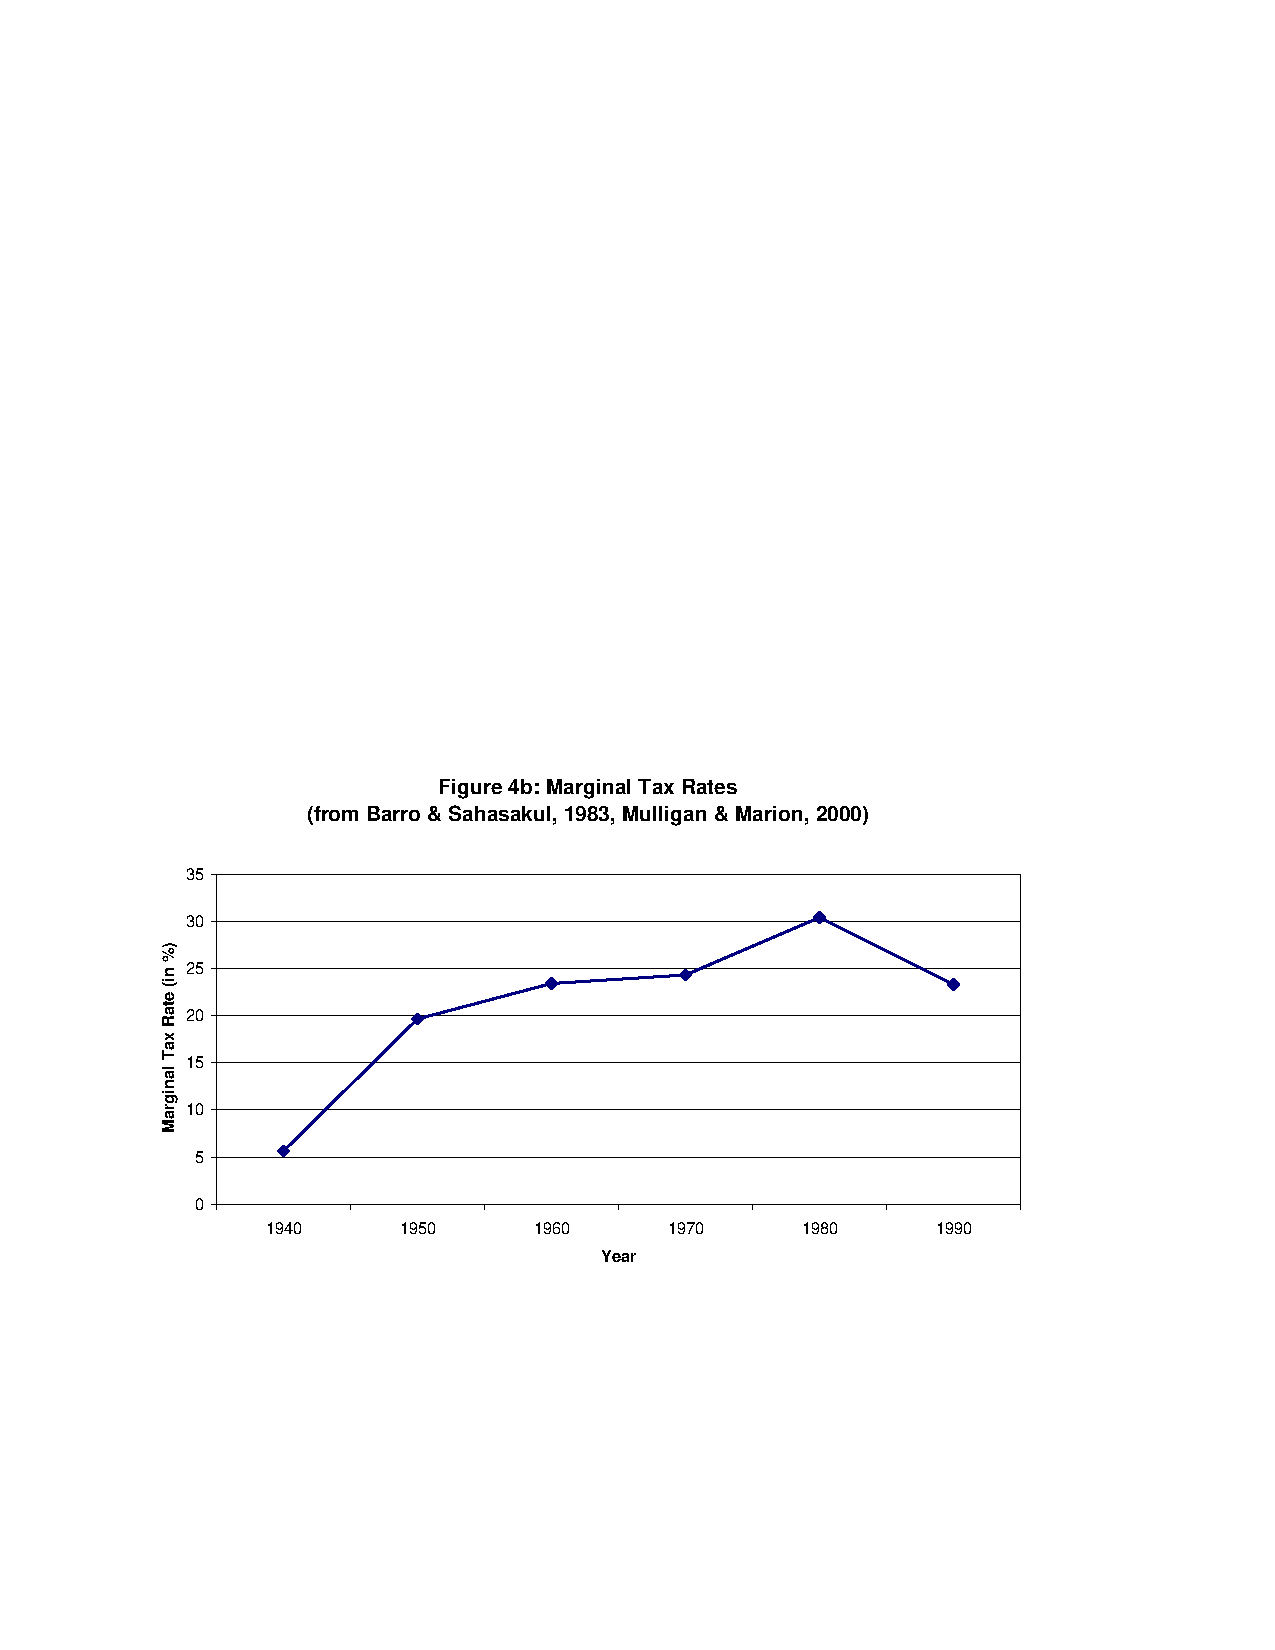
\includegraphics{fig-marginal-taxes}}
\end{center}
\end{frame}
%-------------------------------------------------------------------------------
%-------------------------------------------------------------------------------
\begin{frame}[plain]
\begin{center}
\scalebox{0.75}{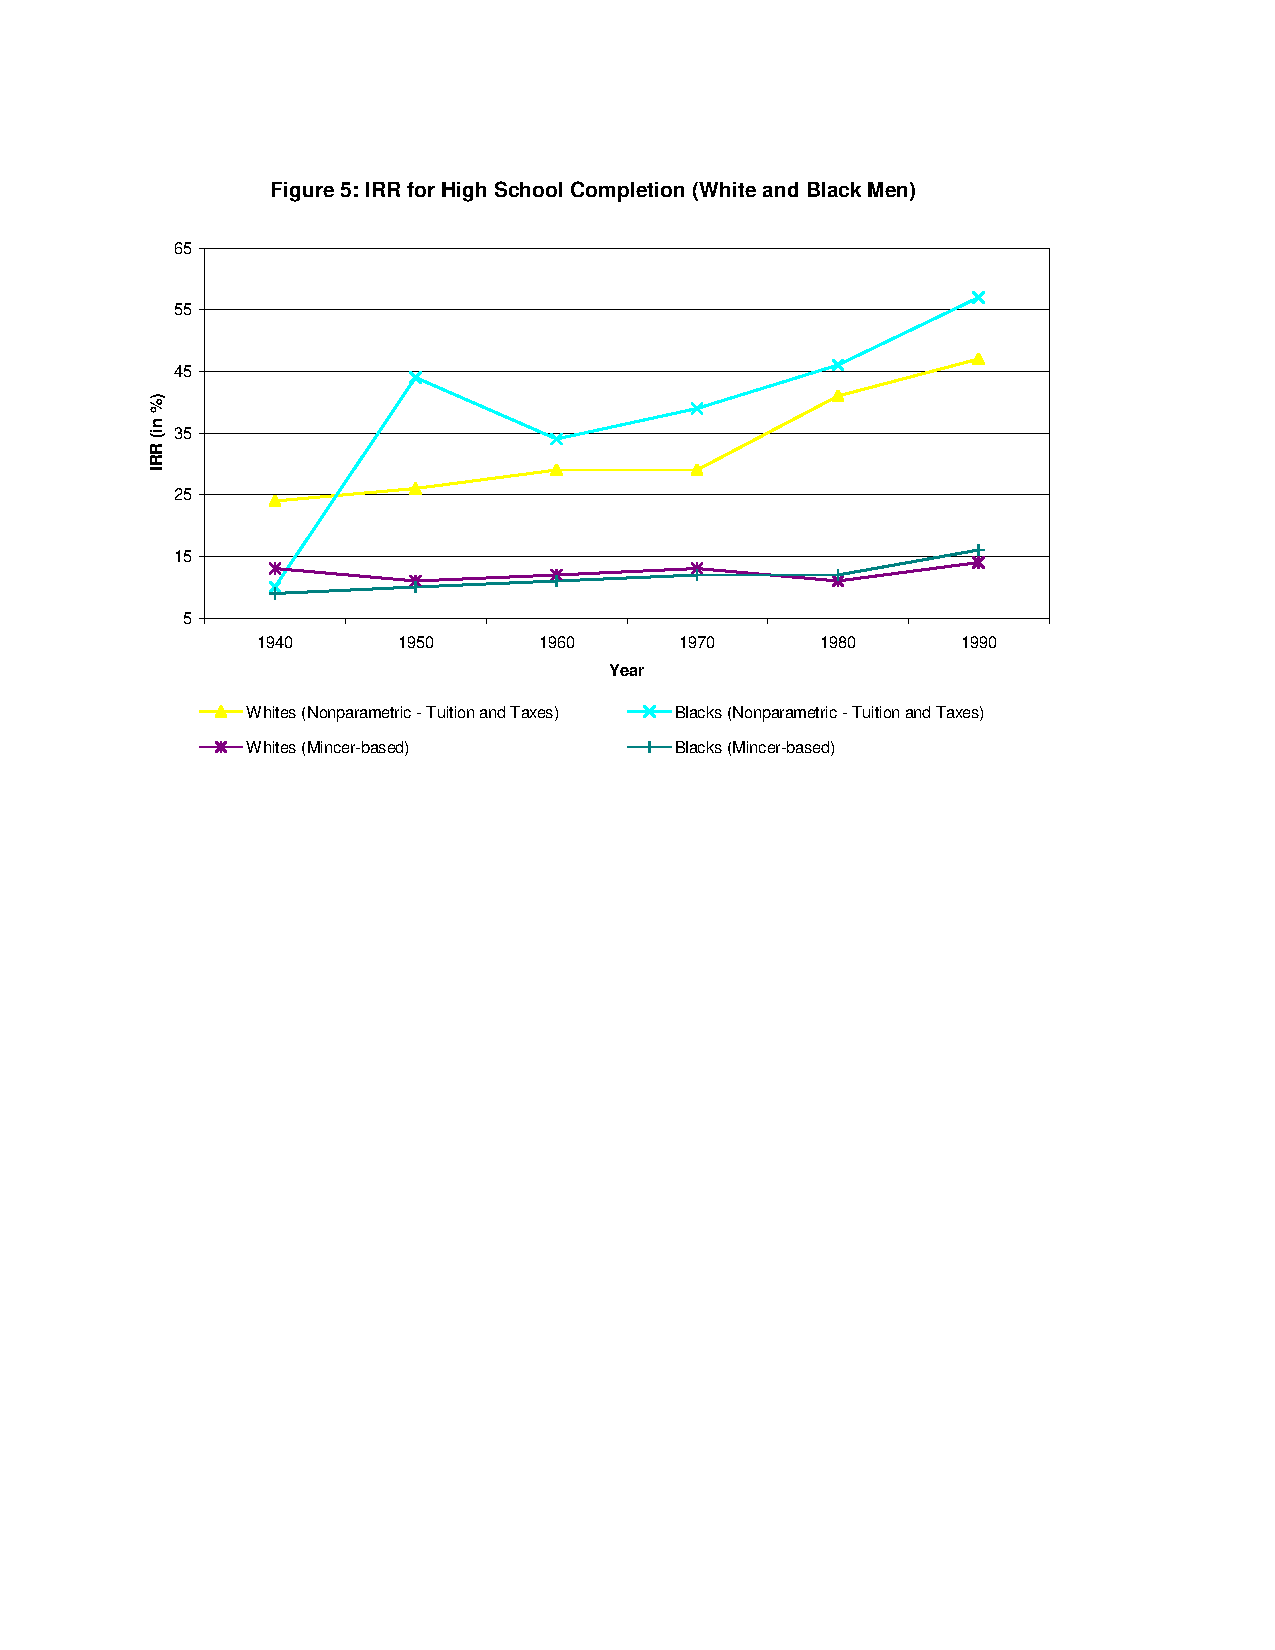
\includegraphics{fig-irr-high-school}}
\end{center}
\end{frame}
%-------------------------------------------------------------------------------
%-------------------------------------------------------------------------------
\begin{frame}[plain]
\begin{center}
\scalebox{0.75}{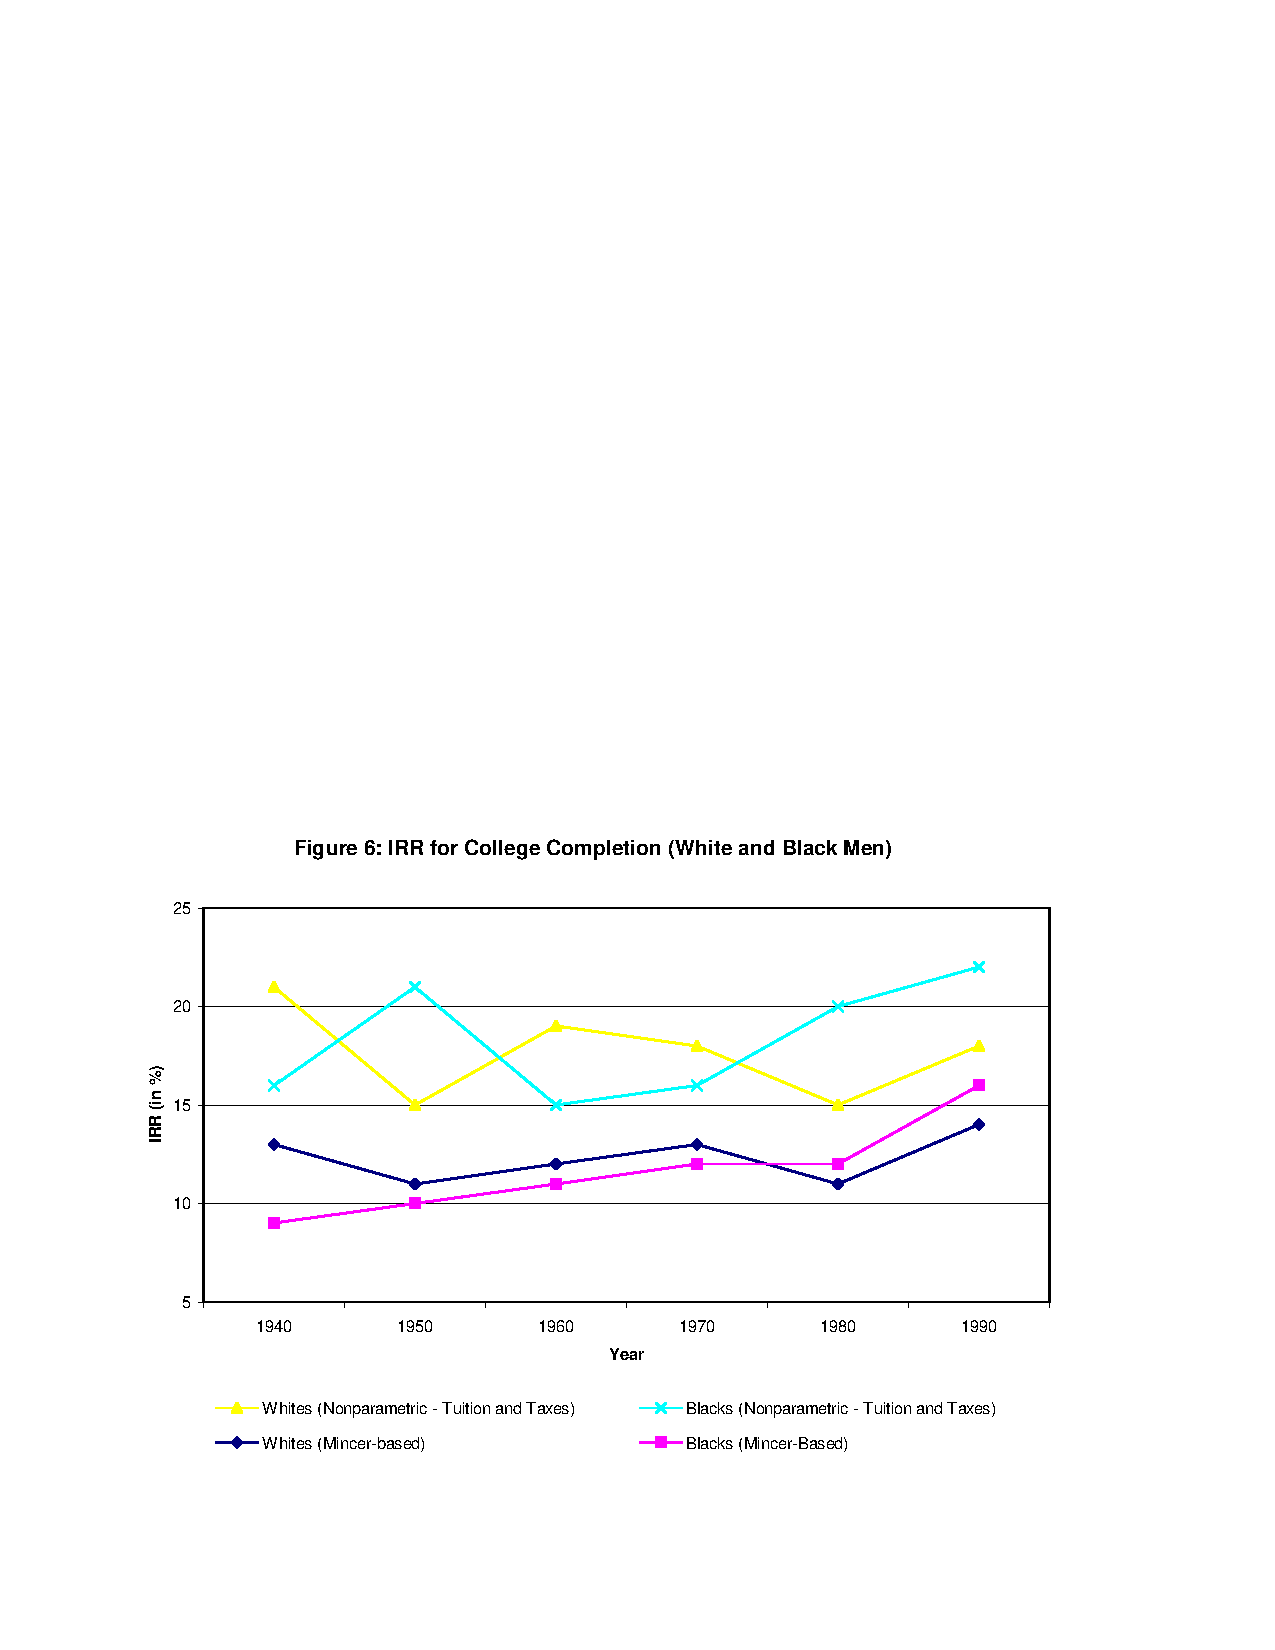
\includegraphics{fig-irr-college}}
\end{center}
\end{frame}
%-------------------------------------------------------------------------------
%-------------------------------------------------------------------------------
